% PyBaMM Conference 2026 — 1-page abstract, V4 (plain-English rewrite)
% Author: Krishna Chaitanya Vaddepally, Turno (Blubble Pvt. Ltd.)
% Deadline: 2026-07-15 UTC
%
% V4 changes vs V3: rewritten in the accepted book-of-abstracts style —
% no equations, no PINN/softplus/collocation/warm-start jargon, no epochs,
% no GPU-time / param-count / optimiser mention. One figure. Reads as a
% battery-modelling talk, not an ML paper.
\documentclass[12pt,a4paper]{article}

% ── Arial-equivalent (Helvetica) as default face; venue requires Arial >= 12pt
\usepackage[T1]{fontenc}
\usepackage{helvet}
\renewcommand{\familydefault}{\sfdefault}

\usepackage[a4paper,top=1.8cm,bottom=1.8cm,left=1.8cm,right=1.8cm]{geometry}

\usepackage{graphicx}
\usepackage{caption}
\usepackage{subcaption}
\usepackage{microtype}
\usepackage{xcolor}
\usepackage[hidelinks]{hyperref}
\usepackage{setspace}
\setstretch{1.08}
\setlength{\parindent}{0pt}
\setlength{\parskip}{0.4em}

\graphicspath{{../outputs/make_agnostic/}}

\usepackage{titling}
\setlength{\droptitle}{-2.6cm}
\pagestyle{empty}

\title{\vspace{-1.0cm}\textbf{\normalsize A neural surrogate guided by
PyBaMM's reaction-limited SEI:\\ 8$\times$ cycling-budget reduction for
used-LFP RUL across three suppliers}}
\author{\normalsize \underline{Krishna Chaitanya Vaddepally}\\[-0.3em]
  \small \emph{Turno (Blubble Pvt.\ Ltd.), India}}
\date{}

\begin{document}
\maketitle
\thispagestyle{empty}

\vspace{-3.6em}
Second-life reuse of used lithium-iron-phosphate (LFP) cells for
stationary energy storage is bottlenecked by characterisation cost.
Cell-by-cell calibration of PyBaMM's~[1] reaction-limited SEI rate
against measured state-of-health (SoH) trajectories is reliable, but
only when at least ${\sim}400$ cycles per cell are available --- below
that, the fitted slope becomes unstable and end-of-life predictions
diverge. For a pack builder receiving a mixed used-cell inventory
across multiple LFP suppliers, this cycling cost dominates repurposing
economics. Recent second-life work~[3] and universal-differential-equation
degradation modelling~[4] have improved calibration quality on similar
cells, but do not shrink the cycling budget itself.

In this work, we train a neural surrogate for cycle-to-cycle SoH
evolution that inherits PyBaMM's reaction-limited SEI ODE~[5] as a
physics prior, grounded in the \texttt{Prada2013} LFP chemistry~[2].
The network is shared across all cells in a cohort, with a small
per-cell adjustment learned jointly so that a single set of
hyperparameters covers cells from different suppliers. The ODE rate
constant is initialised from a linear fit on the short measurement
window and refined alongside the network. Training combines a data
term on the measured window with a physics term that enforces PyBaMM's
SEI rate across the full extrapolation domain.

Applied to 20 used LFP cells from three commercial suppliers
(anonymised A/B/C for confidentiality --- 7, 9, 4 cells respectively),
a single model trained on the first 50 cycles per cell predicts the
remainder of each cell's life with held-out RMSE under 4 percentage
points SoH on all 20 cells (Fig.~1a). Direct linear-slope extrapolation
on the same 50-cycle window diverges: on the deep-second-life
supplier-A cohort, its median error is ${\sim}20$~pp against the
neural surrogate's 3~pp (Fig.~1b). Relative to per-cell PyBaMM
calibration at K=400, our approach reaches the same engineering
accuracy from 50-cycle inputs --- an \textbf{8$\times$ reduction in
required cycling budget, transferring across suppliers without
per-supplier retraining}. In the talk we will discuss the failure
modes of this transfer --- cells whose SoH trajectories violate the
monotonic-fade assumption --- and outline extensions to non-isothermal
operation and time-varying C-rate.

\vspace{-0.8em}
\begin{figure}[h!]
  \centering
  \begin{subfigure}[t]{0.49\textwidth}
    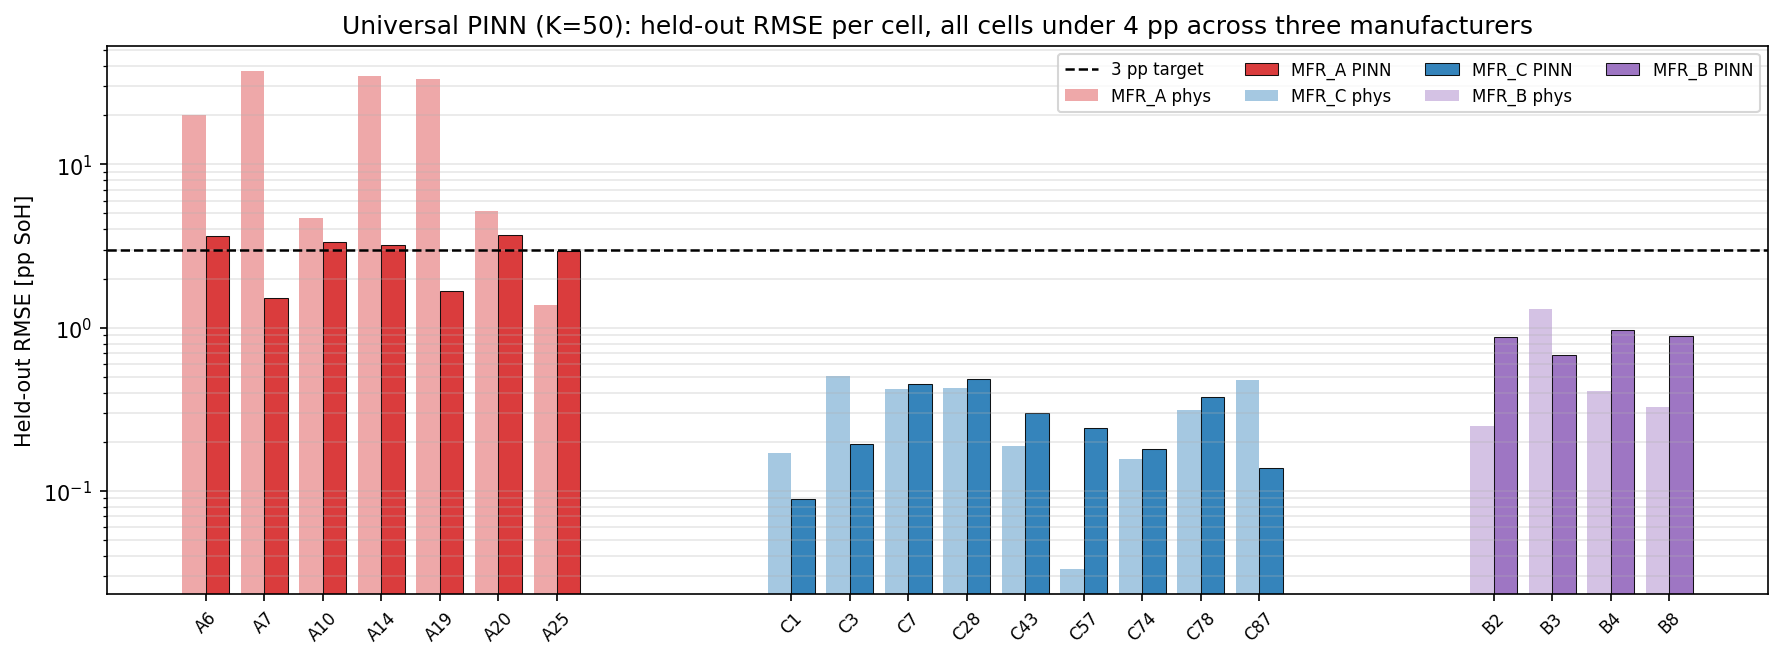
\includegraphics[width=\linewidth]{anonymised_bar_v3.png}
    \caption*{\footnotesize (a) Held-out RMSE per cell across three
      LFP suppliers (log scale). Linear-slope extrapolation towers
      above the 3\,pp target on the deep-second-life supplier-A
      cohort; the neural surrogate stays under 4\,pp on every cell.}
  \end{subfigure}\hfill
  \begin{subfigure}[t]{0.49\textwidth}
    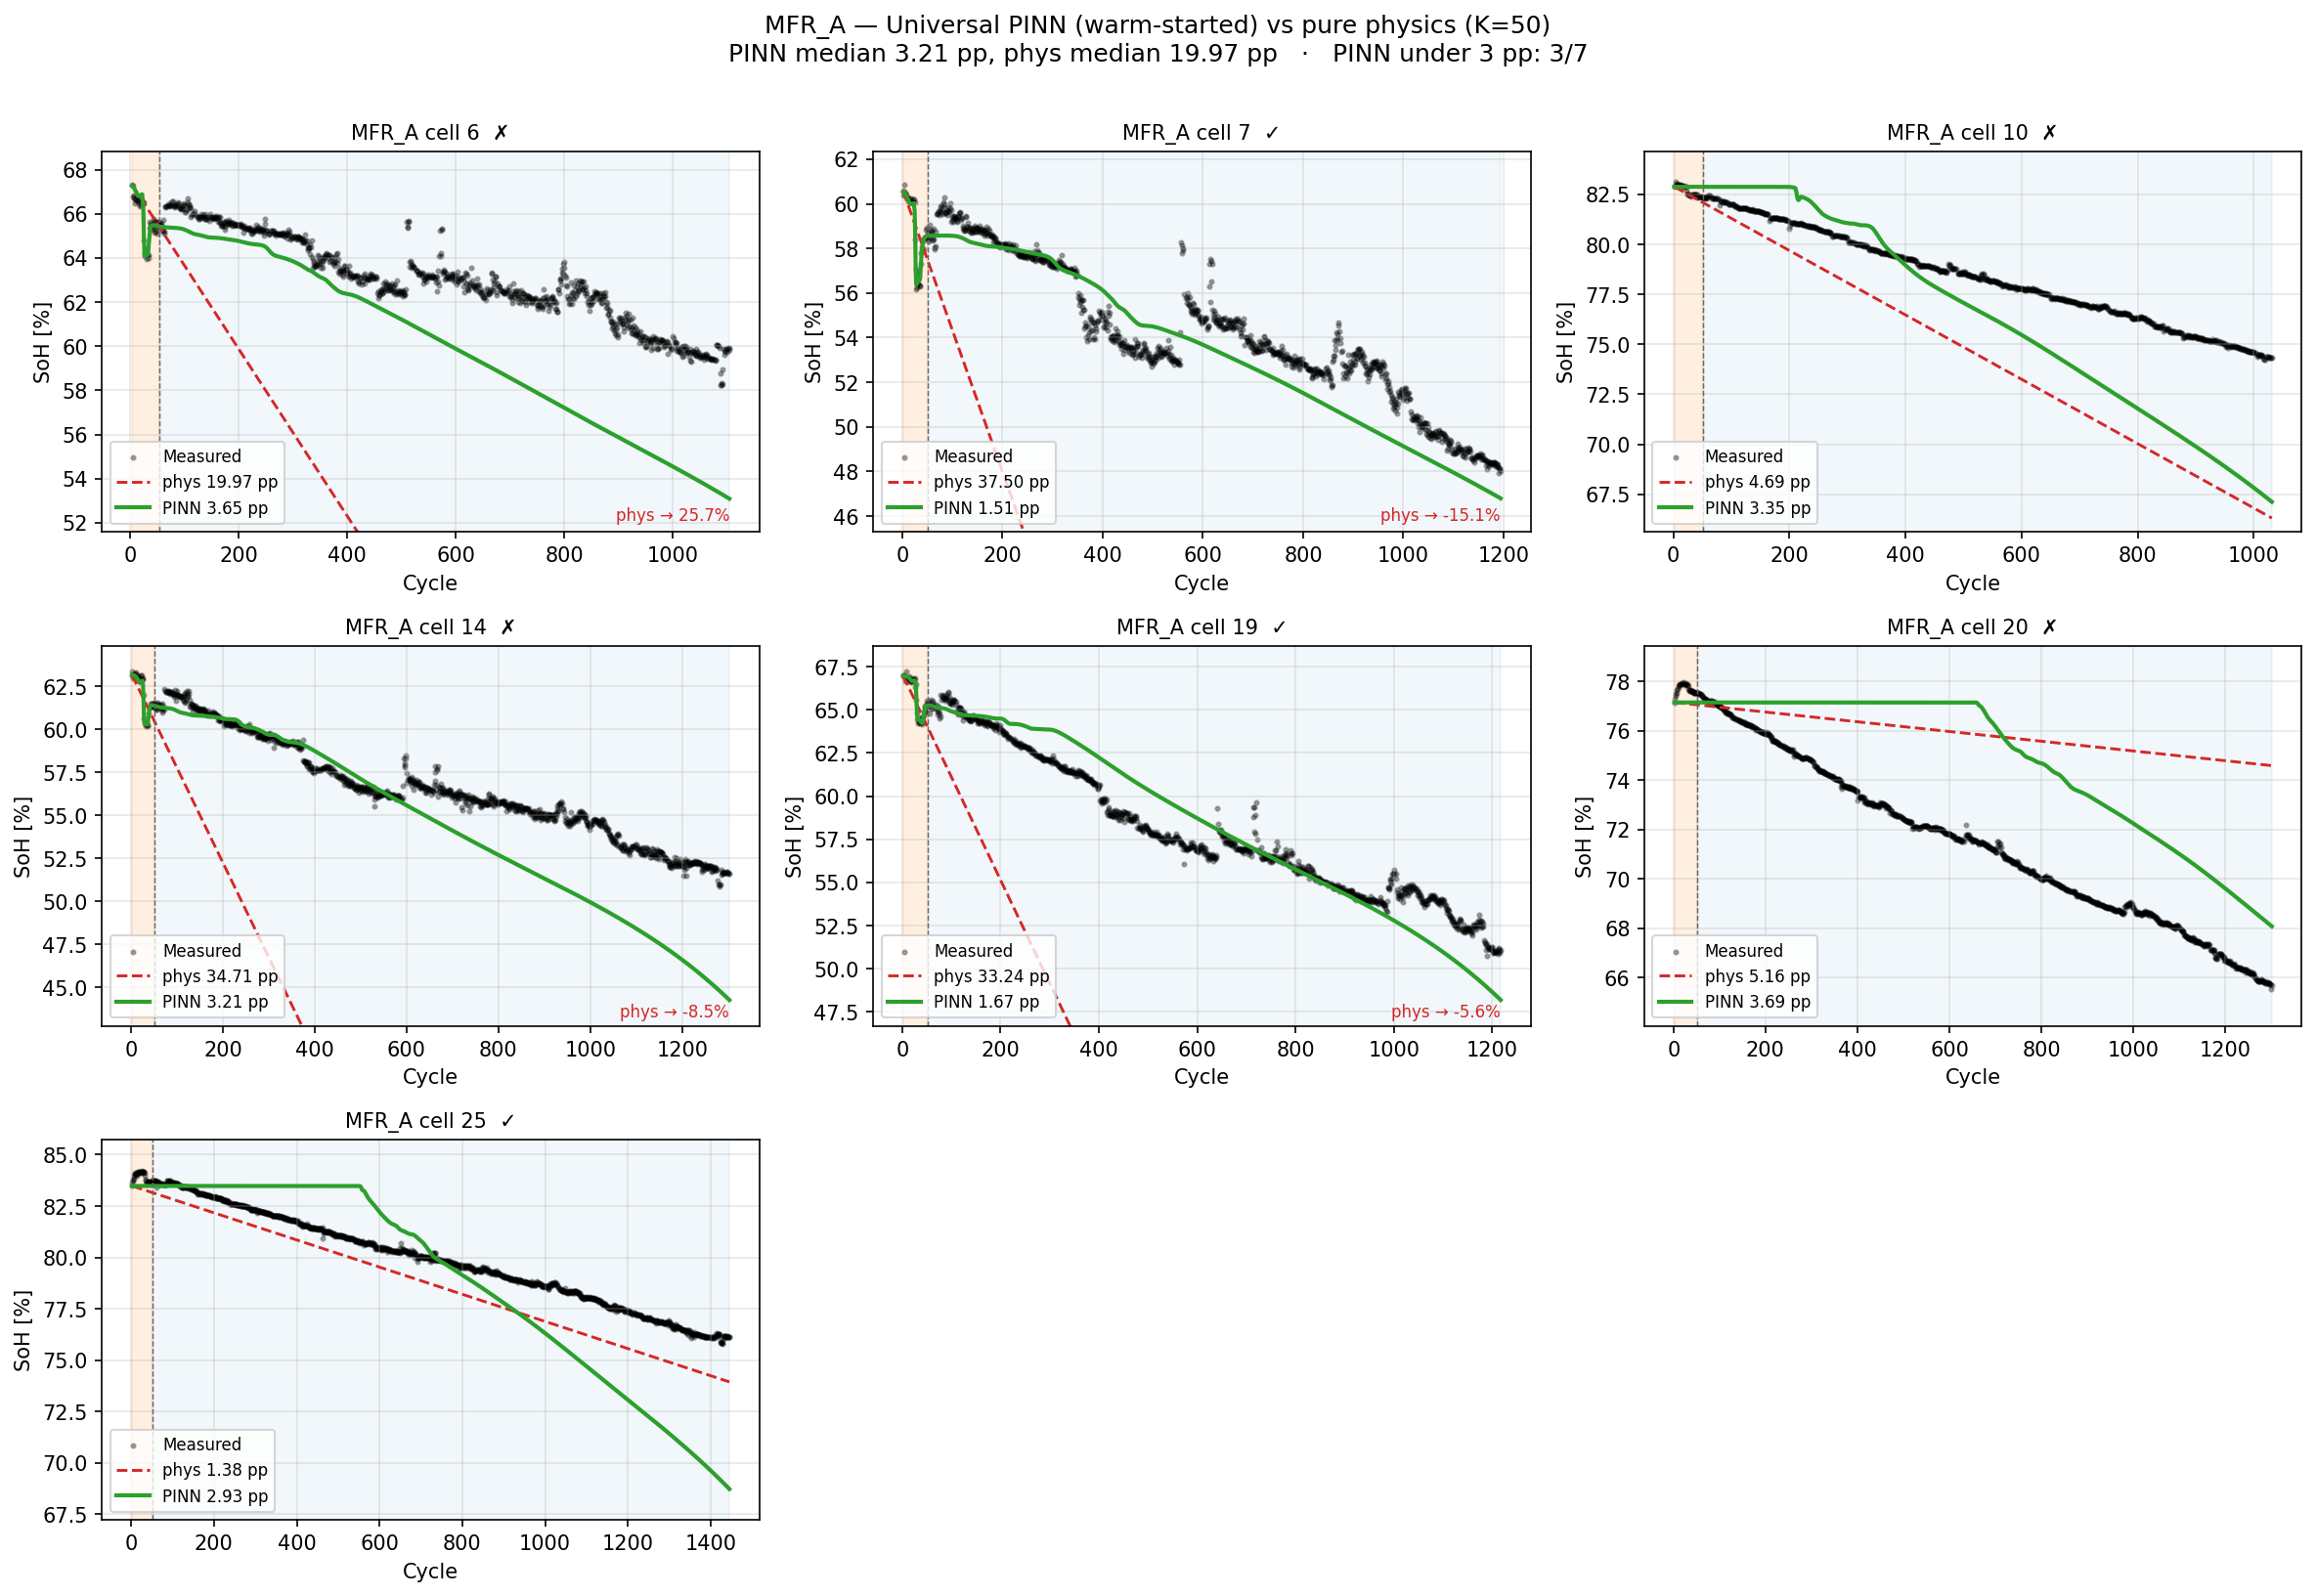
\includegraphics[width=\linewidth]{anonymised_mfr_a_grid_v3.png}
    \caption*{\footnotesize (b) Supplier-A trajectories from 50
      training cycles (orange). Linear extrapolation (red) exits the
      frame with impossible-SoH annotations; the neural surrogate
      (green) tracks measured across 1000+ cycles.}
  \end{subfigure}
  \caption*{\footnotesize Figure 1: Held-out error at K=50 across the
    20-cell used-LFP cohort.}
\end{figure}

\vspace{-0.6em}
{\scriptsize
\noindent\textbf{References.}\;
[1] V. Sulzer et al., \emph{Python Battery Mathematical Modelling
(PyBaMM)}, J. Open Res. Softw. 9(1), 14--21 (2021).\;
[2] M. Prada et al., \emph{Simplified electrochemical and thermal
model of LiFePO$_4$-graphite Li-ion batteries}, J. Electrochem. Soc.
160(4), A616--A628 (2013).\;
[3] O. Ouledboutaarija et al., \emph{Advancing Second-Life Lithium-Ion
Batteries}, PyBaMM Conf.\ 2025 Book of Abstracts, p.\ 19.\;
[4] J. A. Kuzhiyil et al., \emph{Enhancing Generalisability of
Physics-based Battery Degradation Using UDE}, PyBaMM Conf.\ 2025 Book
of Abstracts, p.\ 12.\;
[5] P. Ramadass et al., \emph{First-principles capacity fade model for
Li-ion cells}, J. Electrochem. Soc. 151(2), A196--A203 (2004).
\par}

\end{document}
